%%\documentclass[11pt]{article}

%% Template for a preprint Letter or Article for submission
%% to the journal Nature.
%% Written by Peter Czoschke, 26 February 2004
%%

\documentclass{nature}

%% make sure you have the nature.cls and naturemag.bst files where
%% LaTeX can find them

\bibliographystyle{naturemag}

\usepackage{listings}
\usepackage{color}
\usepackage{caption}
\usepackage{subcaption}
%\usepackage{amsthm,amsmath,amssymb}
%\usepackage{multirow}
\usepackage[pdftex]{graphicx}
%\usepackage{subfigure}
%\usepackage{makecell}
%\usepackage{booktabs}
%\usepackage{array}
%\usepackage{fullpage}
\usepackage{url}
%\usepackage{algorithm}
%\usepackage{algorithmic}
%\usepackage{bm}
%\usepackage{smile}
%\usepackage{mathtools}
%\usepackage{wrapfig}
%\usepackage{lipsum}
%\usepackage{mathrsfs}
%\usepackage{dsfont}
%\usepackage{titling}
%\usepackage{epstopdf}
%\usepackage{multirow}
%
%\usepackage[usenames,dvipsnames,svgnames,table]{xcolor}
%\usepackage[colorlinks=true,
% linkcolor=blue,
% urlcolor=blue,
% citecolor=blue]{hyperref}
%
%\def\skeptic{{\sc skeptic}}
%\newcommand{\sgn}{\mathop{\mathrm{sign}}}
%\providecommand{\norm}[1]{\|#1\|}
%\providecommand{\bnorm}[1]{\big\|#1\big\|}
%\providecommand{\enorm}[1]{| \! | \! |#1| \! | \! |}
%\providecommand{\bemnorm}[1]{\big| \! \big| \! \big|#1\big| \! \big| \! \big|}
%
\renewcommand{\baselinestretch}{1.1}
%
%
%\def\skeptic{{\sc skeptic}}
%\providecommand{\norm}[1]{\|#1\|}
%\providecommand{\bnorm}[1]{\big\|#1\big\|}
%\providecommand{\enorm}[1]{| | |#1| | |}
%\providecommand{\bemnorm}[1]{\big| \big| \big|#1\big| \big| \big|}
%
%\newcommand*{\Sc}{\overline{\cS}}
%\newcommand*{\Ac}{\overline{\cA}}
%\newcommand*{\Bc}{\overline{\cB}}
%\newcommand*{\supp}{\mathrm{supp}}
%
%\DeclarePairedDelimiter\ceil{\lceil}{\rceil}
%\DeclarePairedDelimiter\floor{\lfloor}{\rfloor}



\usepackage[plain]{fancyref}
\makeatletter
\def\mkfancyprefix#1#2{%
\expandafter\def\csname fancyref#1labelprefix\endcsname{#1}%
% plain lowercase
\begingroup\def\x{\endgroup\frefformat{plain}}%
    \expandafter\x\csname fancyref#1labelprefix\endcsname
    {\MakeLowercase{#2}\fancyrefdefaultspacing##1}%
% plain uppercase
\begingroup\def\x{\endgroup\Frefformat{plain}}%
    \expandafter\x\csname fancyref#1labelprefix\endcsname
    {#2\fancyrefdefaultspacing##1}%
% vario lowercase
\begingroup\def\x{\endgroup\frefformat{vario}}%t
    \expandafter\x\csname fancyref#1labelprefix\endcsname
    {\MakeLowercase{#2}\fancyrefdefaultspacing##1##3}%
% vario uppercase
\begingroup\def\x{\endgroup\Frefformat{vario}}%
    \expandafter\x\csname fancyref#1labelprefix\endcsname
    {#2\fancyrefdefaultspacing##1##3}%
}
\makeatother

\mkfancyprefix{thm}{Theorem}
\mkfancyprefix{lem}{Lemma}
\mkfancyprefix{prop}{Proposition}
\mkfancyprefix{cor}{Corollary}
\mkfancyprefix{def}{Definition}
\mkfancyprefix{cl}{Claim}
\mkfancyprefix{ss}{Subsection}
\mkfancyprefix{alg}{Algorithm}
\mkfancyprefix{ass}{Assumption}

\title{Brainconductor: An open science platform for the development of
neuroimaging
data analysis tools}

%% Notice placement of commas and superscripts and use of &
%% in the author list

\author{Kevin Lin$^{1*}$, Haixiao Du$^{2*}$, Huazhong
Yang$^2$, Yu Wang$^2$, Han Liu$^3$}

\begin{document}

\maketitle



\begin{affiliations}
\item Department of Statistics, Carnegie Mellon University,
Pittsburgh, PA 15217 USA
\item Department of Electronic Engineering, Tsinghua University, Beijing, China,
100084
\item Department of Operations Research and Financial Engineering, Princeton
University, Princeton, NJ 08544 USA
\item[*] These authors contributed equally to this work
\end{affiliations}

\begin{abstract}
    Brainconductor project is a project parallel to Bioconductor. Like
Bioconductor, Brainconductor is an open platform for sharing neuroimaging data
and R-based data analysis software. Brainconductor aims at promoting
interdisciplinary collaboration between neuroscientists and
statistical scientists, bringing state-of-the-art statistical methodologies and
toolboxes into neuroscience, and enhancing the reproducibility of remarkable
research results. We describe details of our motivations, goals, methods, and
the difference between Brainconductor and related neuroinformatics projects.
Finally, we present some working instances to better explain the advantages of
Brainconductor.
\end{abstract}


Modern statistics aims to infer information from high-dimensional data
and has progressed significantly over the last decade.
However, two obstacles currently hinder the
application of these methods to large-scale neuroimaging data
in practice. 
First, domain-specific expertise and computational power is needed to handle
the various data file types and to manage the storage
of these large-scale datasets. Second, the pipeline of a typical
neuroimaging analysis can span multiple software platforms such as FSL, AFNI,
Python, Matlab and R. This decentralized workflow hinders a reproducible 
analysis and discourages new researchers from learning all the
necessary tools across different platforms.
The Brainconductor project is an open-neuroscience
initiative to address
these obstacles.
As the neuroscience community expands upon open-access
datasets such as the  International Neuroimaging Data-Sharing
Initiative Project (INDI), comparable advances in
open-neuroscience platforms are required
for high
throughput, computationally efficient statistical models
to handle high-dimensional data in this big data era.

%The cooperative trends creates new challenges.
Our goal is to %, and the foremost of all is to
build a knowledge hub and interdisciplinary community by connecting
neuroscientists and statisticians.  Neuroscientists
drive the scientific process by collecting new data and constructing focused
experiments. Non-invasive imaging techniques have gained popularity to
investigate the influence of phenotypic variation
on brain connectome\cite{sporns2005human,sporns2011human},
the coordination among different brain regions when users perform
tasks {\color{red}wording and citation},
the structural architecture of the brain {\color{red}citation} and many more. 
These include structural and functional MRI,
diffusion tensor imaging (DTI), and Electroencephalography
(EEG).
On the other hand, statisticians bring new statistical methods
designed to address the high-dimensional, large-scale and complex
data. Such techniques can be divided broadly into
two categories:
feature extraction (i.e., estimating the connectome or structural 
properties of the brain, summarizing
a parcellation of voxels into a single statistic,
identifying relevant biomakers associated with changes in the connectome architecture)
and uncertainty assessment (i.e., testing for significant difference
between the connectomes of two populations, determining if 
an extracted feature is due to chance).
We strive to help enable the ease of collaboration between these two communities.
While the neuroscientist will benefit from the modern techniques to
analyze these datasets, the statistician
will benefit from the lowered barrier-to-entry
due to the  simplified processes of data acquisition, data management, and data
sharing. These are summarized in \Fref{fig:overview}.

\begin{figure}[tb]
\centering
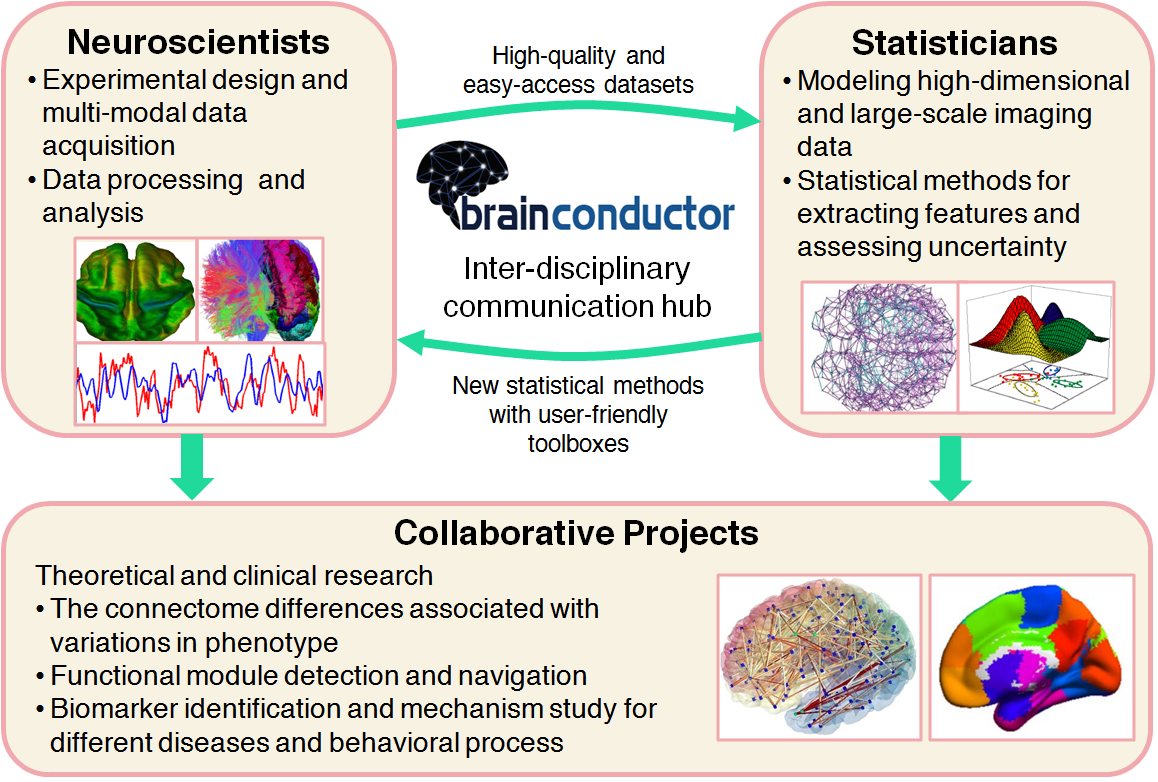
\includegraphics[width=400pt]{fig/brainconductor/Brainconductor_overview.png}
\caption{Specialties of neuroscietists and statisticians and the potential
topics to explore in collaborative projects.}
\label{fig:overview}
\end{figure}

Towards this end, we propose the Brainconductor project, an integration of
high-quality and easy-access datasets, and user-friendly software for both
neuroscientists and statisticians. Brainconductor is a project parallel to
Bioconductor. In the past tens of years,
Bioconductor\cite{gentleman2004bioconductor} made a great contribution to the
progress of
the human genome research because of its transparency, pursuit of
reproducibility, and efficiency of development. Moreover, the open-source
developing architecture of Bioconductor based on R language provides facility to
take advantage of the mature statistical packages rather than re-implementing
functionality. In future neuroimaging studies, an open-source platform is of
necessity to produce collaborative creation of extensible computational tools
and enhance the reproducibility of research results.




This desire has already  %requirement
inspired one of the most prominent projects, Neuroimaging
Informatics Tools and Resources Clearinghouse (NITRC).
NITRC is a resourceful repository collecting popular neuroimaging tools
designed for the preprocessing,
analysis, and display of neuroimaging data, such as
SPM\cite{penny2011statistical}, FSL\cite{jenkinson2012fsl},
FreeSurfer\cite{fischl2012freesurfer} and AFNI\cite{cox1996afni}. NITRC also is
an open repository for many
data sources such as
Alzhelmer's Disease Neuroimaging Initiative (ADNI) and the
1000 Functional Connectome Project (FCP).
However, as successful as NITRC is, there are fundamental
drawbacks from both the developer and user perspectives.
From the developer perspective,
NITRC provides little guidance on effective software
development.
This results in two consequences. First, a large amount of
effort is spent on implementing functions that have
previously been developed by other independent teams. Second,
without establishing an universal file format,
developers on NITRC have to either
write analysis functions for specific file types or spend tremendous
efforts to handle all file types.
For example,
most data sources proffer raw data in the standard industrial DICOM
format, but most of the software packages work on NIfTI or ANALYZE formats.
From the user perspective, there are also key obstacles.
First, software on NITRC are based on different programming models and
processing pipelines and have different interfaces.
Hence, investigators always need lots of training sessions to
learn how to install and use these tools. Second, many statistical
analysis software require a 2D matrix where each covariate
represents a column and each sample represents a row. Since neuroimaging
data is typically represented as a 4D object, new users often
struggle to convert their data into a representation suitable for
most statistical methods. These concerns are summarized in \Fref{fig:nitrc}.

\begin{figure}[tb]
\centering
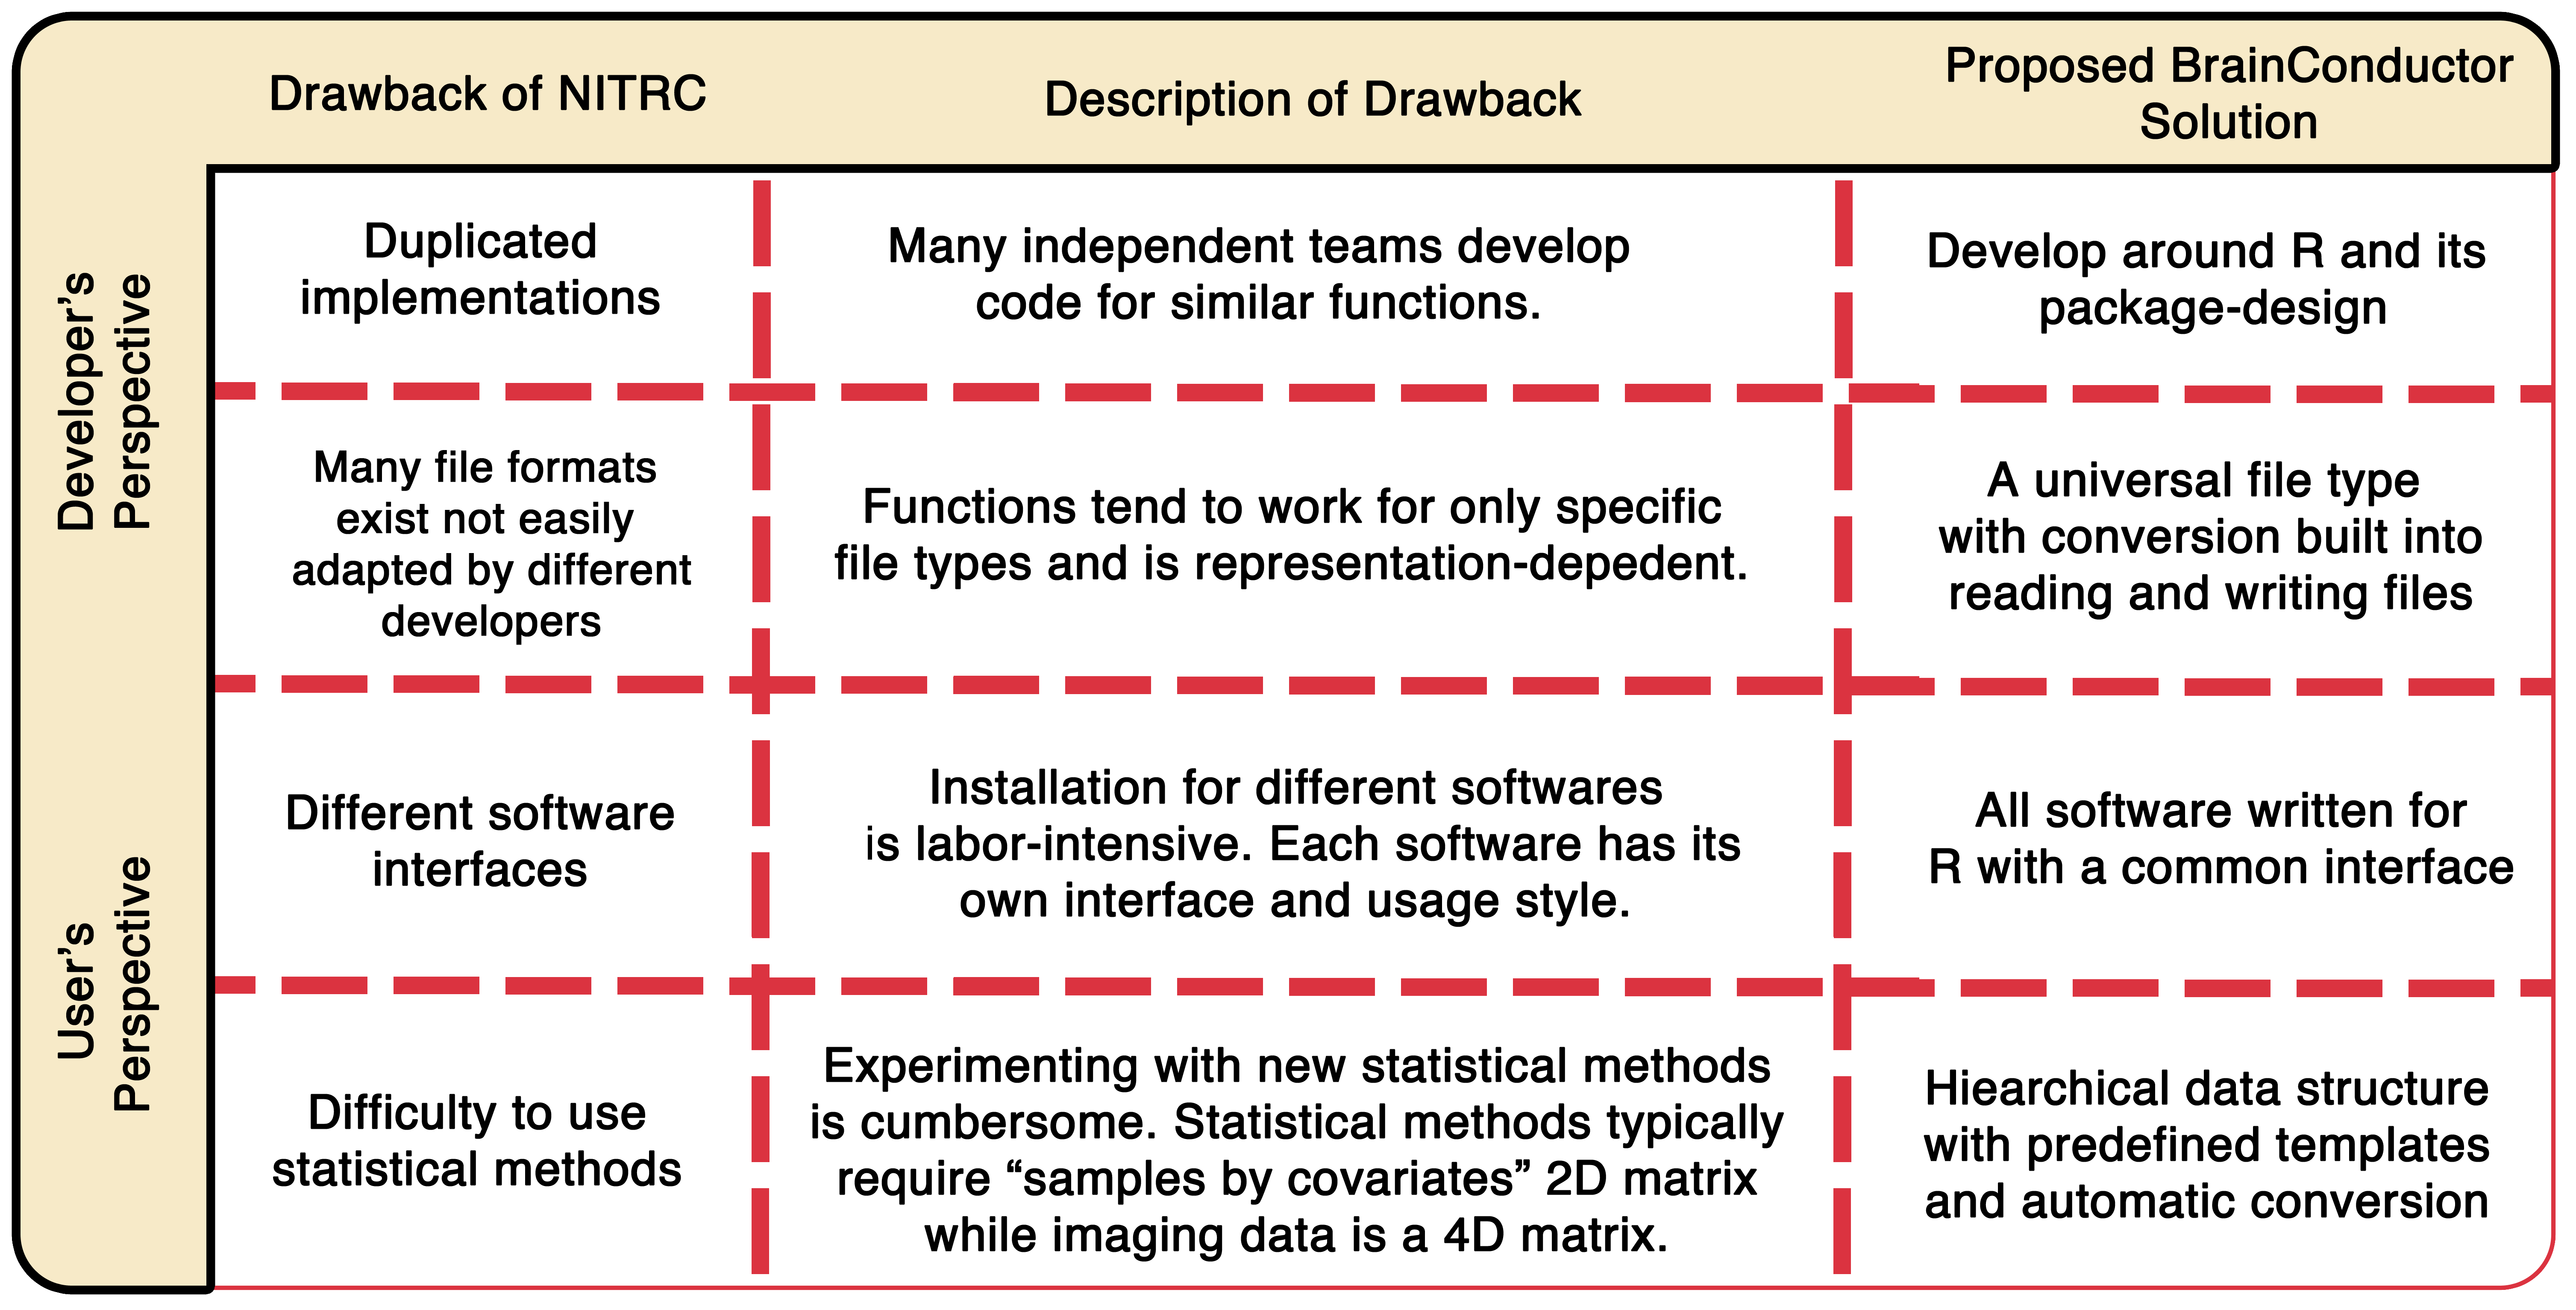
\includegraphics[width=400pt]{fig/brainconductor/brainconductor_nitrc_chart_v2.png}
\caption{Drawbacks of NITRC framework, description of the drawbacks and proposed
solution in Brainconductor. {\color{red}Need to fix alignment}
}
\label{fig:nitrc}
\end{figure}


The Brainconductor project serves two fundamental goals. In connectome-wide

association studies, one fundamental goal is to relate differences between the
macro- and microarchitecture of the human connectome to phenotypic variation among
individuals\cite{milham2012open}. Towards this end,
in our initial release of Brainconductor, we focus on an open-neuroscience
solution to manage resting-state fMRI data and study its
subsequent brain connectivity patterns. {\color{red}Do we want to explicitly say
this?}
However, there are many scientific goals to a field as broad as neuroscience,
and we plan to support all types of neuroimaging analyses within Brainconductor
with the help of the community.
For example, in imaging genetics, the ultimate goal
for Brainconductor project is to identify biomarkers and help early diagnosis
for a variety of neuropsychiatric disorders. This will involve an
integration of genomics and neuroimaging data and expansion of Brainconductor
in the future. Our work paves the foundation for this long-term community 
project.


\section{Merits of Computational Strategy}

\subsection{Functionality of R.}
The existing features and communities around a language dictate
its usage and accessibility. As stated before, we are
interested in problems related to data management, mining and analysis
associated with neuroimaging technologies. This orientation requires
a programming environment which is able to foster
efficiency for software development, allow
streamlined and reproducible research and simulate
interdisciplinary communication and cooperation.

To meet these requirements, we chose R as the basic programming
modal for Brainconductor project. Our rationale closely follows
the reasons adopted in Bioconductor which we summarize
here\cite{gentleman2004bioconductor}.
First, R is an accessible high-level language with
good numerical capabilities allowing quick prototyping of new statistical
computational methods. This allows for a low learning curve for
incoming researchers, rapid experimentation of
new statistical ideas, and a shorter development cycle.
Second, R has a packaging protocol for different software
modules that can be developed individually and distributed easily. The
packaging system of R enables a worldwide collaborative construction of the
Comprehensive R Archive Network (CRAN) with a wide range of
high-quality and well-documented statistical and visualization software
packages. These hundreds of packages are independently developed for specific
objectives, but the objective-oriented programming style of R guarantees the
robust interoperability of packages for more complicated applications. All of
these characteristics of R would decrease development efforts and release time
for reliable software for neuroimaging data analysis.
Third, R also provides
support for high-performance\cite{buckner2010gputools} and parallel
computing\cite{schmidberger2009state},
and interfaces to communicate with specialized code
written in lower-level languages.
Finally, the community of R is
consisted of thousands of active users and developers including biologists,
mathematicians, and engineers. The community provides a natural bridge to
connect the neuroscientists and statisticians. This is much in line with the
intention of the Brainconductor project and is the most important motivation for
our selection of the R language.


\subsection{Hierarchical Data Structure.} The Brainconductor
project began with significant investment in the infrastructure construction for
software development by formulating the standard for general data structures of
neuroimaging data.
The data structures are assembled to form our hierarchical
data structure called NIdata.
Our general data structure provides designers with the 
convenience of designing code around one interface
while enabling users to have the flexibility to store
only the data they are interested in their study.

Currently, the most common file format is NIfTI.
NIfTI is a product of the Data Format Working Group
(DFWG) from the Neuroimaging Informatics Technology Initiative project. It
contains both the header information about the data acquisition
parameters and neuroimaging data as a 4D matrix.
Currently, the oro.nifti R package defines the `nifti'
S4 class in R to manage NIfTI files. However, there are two drawbacks
of this file format that could be encountered by analysts. 
First, the NIfTI file format is not aligned with
most statistical analyses. Typically,
phenotype information is stored separately in a different file. Hence, users must use a third-party software to determine the subjects in each cohort before performing the population-level case-control study. Likewise, many
statistical
methods (i.e., regression and classification) require as input a 2D matrix organized by samples and covariates. This results in users often writing 
their own code to translate the 4D brain data 
into a compatible 2D format.
Second, neuroimaging
data files often contain a large amount of
redundant information not relevant for a particular
analysis.
For example,
the analysis of fMRI data primarily focuses on the gray matter, while the
processing of diffusion weighted MRI focuses on the white matter region. The Human Connectome Project (HCP) faced a similar problem which they
overcome by defining the
CIFTI
file format and grayordinates, a combined cortical surface and subcortical
volume coordinate system\cite{Glasser2013The}. 


We define an S4 `NIdata' class based on the NIfTI format
in our Brainbase package as
the general data structure to resolve these problems. We designed
the data structure hierarchy to enable convenient integration with
downstream
statistical analysis as well as to optionally store only portions of the
data that the user is interested in.
At its core, the NIdata class is a generic file type split into
six slots to store the following information: 1) the neuroimaging data,
2) phenotype
information, 3) specifics of scan sessions,  4) an optional subject ID,
5) a ``wildcard" extra slot for any other information that user
wants to store such as statistical results,
and 6) text-based comments or notes associated with the data that
investigators might document. While the
S4 class provides an initial structure for storing
phenotype and scan information, users have the flexibility to disregard or
modify these templates before reading the data into R.



Most of the engineering of the NIdata class revolved around a more suitable
representation of the neuroimaging data to overcome the potential
drawbacks of the NIfTI format. Like in the CIFTI file
format\cite{Glasser2013The},
NIdata can automatically convert neuroimaging data (a 4D matrix)
into a 2D (potentially sparse) matrix where each
column represents a different voxel
in the brain and each row represents
a different sample from the series (i.e., time series in fMRI, directional
series in DTI). To ensure that the column indices are
compatible across different NIdata objects, we define generic templates in the
Brainbase packages that dictate which voxel positions are assigned to which
columns.
These templates are associated with brain masks and the corresponding tissue
priors. 
For instance, one of the templates we provide is the MNI 152 brain masks and
tissue priors typically found in FSL.
If users want to keep only voxels corresponding to gray matter, all the column
indices associated with non-gray matter will be `zero'-ed out to save storage.
Moreover, if users want to perform a
region-of-interest or parcellation-based analysis, we provide
additional functions to change the template and perform the data extraction.
For example, using the Automated Anatomic Labeling (AAL) parcellation\cite{tzourio2002automated},
users can reduce the voxel-level data into a parcel-level data where the fMRI
signal of each parcel is determined the mean or the first principal component, the two most
common data-extraction methods.

We discuss the hierarchical nature of the NIdata class. To implement the strategy mentioned
above, we chose to create a collection of various S4 data classes, most of which are combined and used
interchangeably in the NIdata class. The S4 objects in R use an object-oriented approach to class design
which enforce consistency within the superclasses and subclasses. Our NIdata data structure consists of
various nested subclasses, giving rise to the hierarchy. 
The
schematic displaying the input of data to the end NIdata representation
is shown in \Fref{fig:fileformat}. We have also designed multiple functions to extract
desired components of this hierarchy so users are not required to learn the hierarchy in order to
take advantage of the NIdata class.

We lastly mention that users have a wealth of flexibility on how to manipulate the NIdata
objects with aid of our other functions. 
First, to ensure that our 2D representation of neuroimaging data retains the
spatial information of each voxel, the Brainbase package provides
an R S4 object containing the mapping of voxel location to column index and
a list enumerating the column indices of neighboring voxels for each voxel
location. Hence, we can convert our 2D representation back to its original
4D representation to accommodate past software requirements if needed.
Thanks to this flexibility, software developers can
implement algorithms operating directly on the 2D representation in
NIdata without worrying about representation-conversion. This also allows users 
to convert between NIdata and NIfTI classes easily. Second, users can use any
templates to process and store NIdata objects. While we have mentioned several templates
provided by the Brainconductor package, users can create customizeable templates. 
This can be done via the reslicing
functions
we provide based on the fslr package. 

\begin{figure}[tb]
\centering
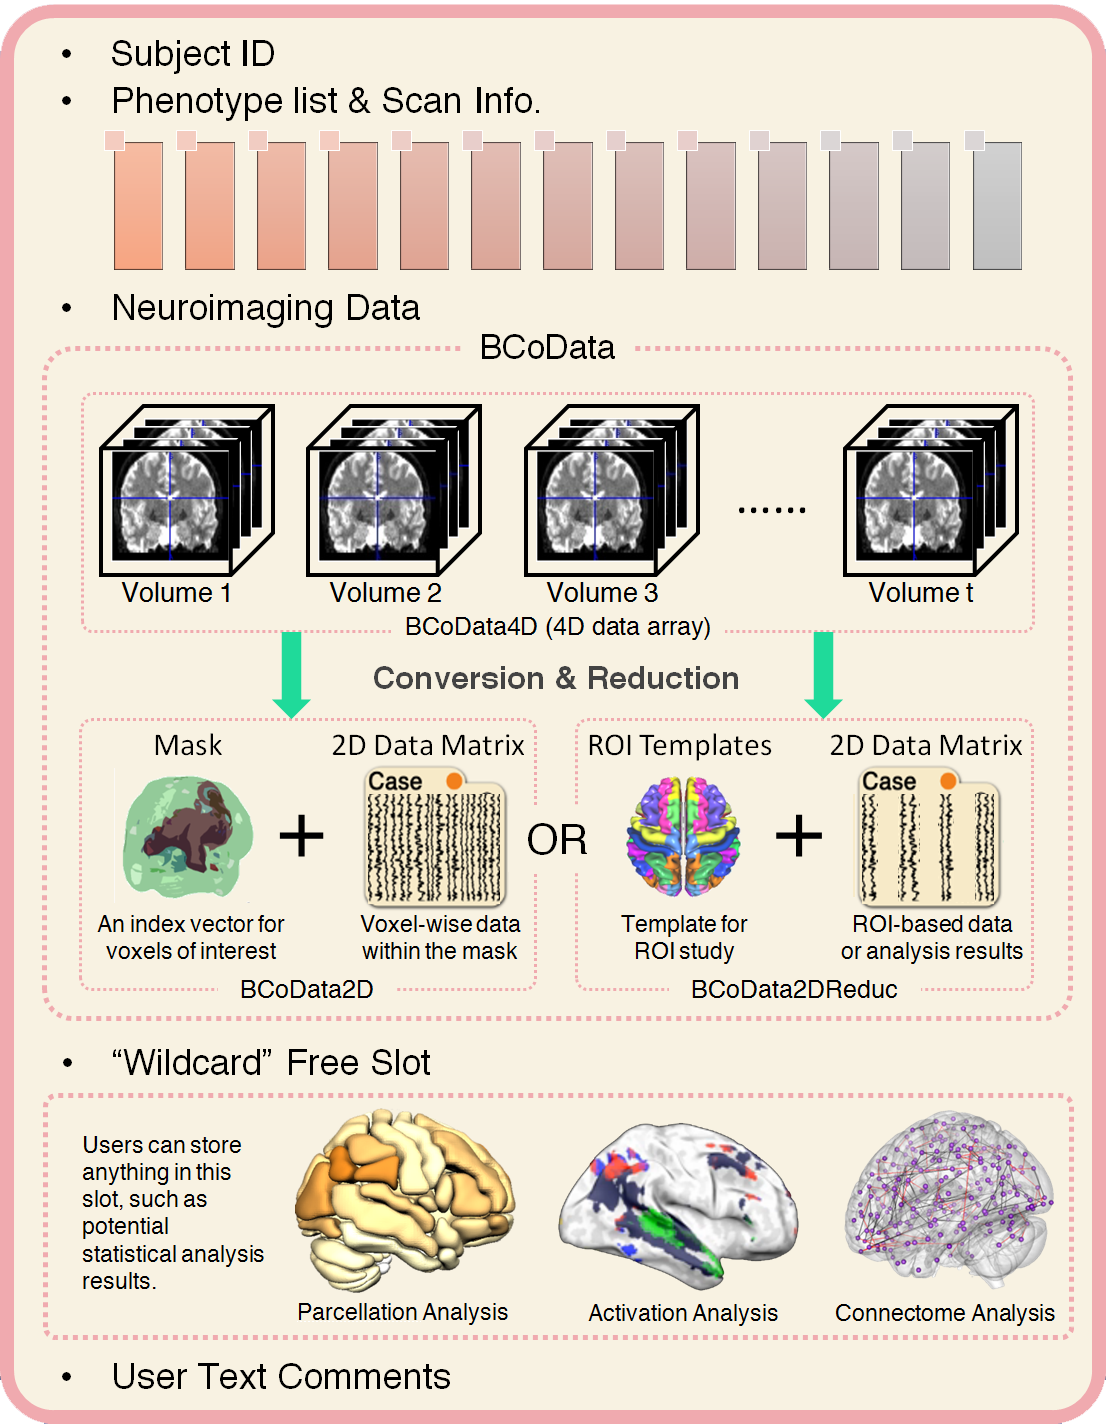
\includegraphics[width=250pt]{fig/brainconductor/NIdata.png}
\caption{Schematic of the hierarchical data format. The top-most bullet represents
the slot for the Subject ID. The next bullet represents the slots for the user-defined
phenotype information and scan info (i.e. from the NIfTI header). Next, the neuroimaging
slot represents a hierarchical data structure where data can be stored as 4-dimensional
matrix (BCoData4D), as a 2-dimensional matrix where each column represents a voxel in
the mask (BCoData2D) or as a 2-dimensional matrix where each column represents a
summary of each region of interest (BCoData2DReduc). The next slot represents a wildcard
where users can store anything of relevance such as analytical results. The last
slot is for users to write any notes for future reference.}
\label{fig:fileformat}
\end{figure}


When designing our NIdata file format in R, we kept the tradition of using S4's
pass-by-value system rather than using an pointer-based system to
pass-by-reference.
A pass-by-reference system would be beneficial as R would not need to 
create local copies of massive neuroimaging data every time it is passed into a
function. While there are R packages to help developers
code using pointers\cite{bengtsson2003r}, there would be a 
considerable burden on future developers to these new coding methods.
Instead, we chose to keep the simplistic S4 system and design the hierarchical
data structure to reduce the memory requirements for storing each NIdata object.

{\color{red}Some concrete numbers of how much memory is saved}

\subsection{File Conversion.}
For developers to write functions using our NIdata class, we need to provide
suitable functions to read different input file types into objects of NIdata
class as described in the previous section. Here, We discuss three popular file
types in current use, DICOM, NIfTI and ANALYZE.

DICOM is the standard industrial
format for raw data directly collected from an imaging device. The DICOM format
is very broad and very sophisticated. In brief, each .dcm suffix file contains a
number of attributes, including not only the image pixel data but also large
amounts of meta-data information about the subject, imaging devices and settings
during data acquisition.

However, DICOM datasets are redundant, ascribed to the storage of massive
numbers of small files. This is due to each image slice stored as a separate
file. ANALYZE and NIfTI-1 formats are more widely employed in the neuroimaging
community. An ANALYZE format document is composed of one ``hdr" file and one
``img" file. The former contains information about the acquisition settings,
while the ``img" file contains the image data. NIfTI was released as an
extension
of the ANALYZE format. The NIfTI data format merges the header and image
information of ANALYZE document into one file (.nii) and enables extending of
the header information. The NIfTI format has alleviated problems with data
storage and sharing across diverse centers, and became one of the most popular
neuroimaging format recently.

Brainconductor offers functions to read all these data format
based on existing software in the oro.nifti package. We
provide a generic function that handles all of these file types and read data
into the desired NIdata object.
We noticed that the oro.dicom package was difficult to use for new users, so
we altered the implementation of how DICOM files are converted into NIfTI 
files. An example of the conversion using oro.dicom compared to a conversion
based on specialized software such as MRIcron\cite{rorden2011mricro} is
shown in \Fref{fig:dicom}.
%{\color{red} TODO: The conversion from DICOM to NIfTI is not well implemented.
%We based on mature
%software dcm2nii (from MRIcron?).}

\begin{figure}[tb]
\centering
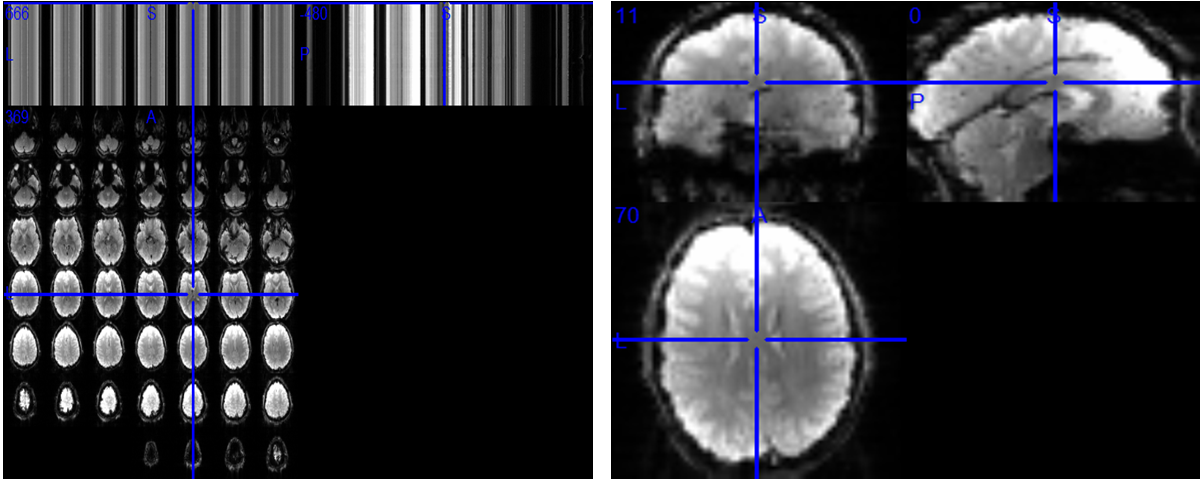
\includegraphics[width=400pt]{fig/brainconductor/dicom.png}

\caption{Comparison between conversion functions from oro.dicom package (left)
and from our Brainbase  package (right).  Our function showed better
compatibility  with widely-used visualization tools such as MRIcron.}
\label{fig:dicom}
\end{figure}

\subsection{Software Distribution.}

All software distributed by Brainconductor is in the form of R packages abiding
to our NIdata structure. This
simplifies software delivery, usage and maintenance but puts a burden on the
developers
to learn how to write R packages, documentation and test cases.

As seen by the success of CRAN and Bioconductor, the packaging system lies
at the heart of why R has been a successful language. We follow their examples.
Changes are tracked using a central, publicly readable Subversion software
repository
so the details of all changes are fully accessible via Subversion.
Simultaneously, since
R itself is continually changing to improve performance and functionality, all
packages
in Brainconductor undergo testing monthly. These required tests are designed by
the
developers themselves and is performed in an automated fashion to ensure
all code examples and unit tests run without errors.

For developers to submit their software to Brainconductor for others to use,
we have designed a specific ``Developers'' section of our Brainconductor website
to guide the process. The package guidelines revolve around usage-oriented
documentation and understanding the input and outputs of each parameter.
 Once
a package is submitted, feedback is given to revise the code or the package is
accepted.
From then on, the package will be available on the
development branch of the project and be part of in the next release of
Brainconductor.
We expect releases to be made every 6 months.
Each package has a designated maintainer responsive by email address and reacts
to
errors, bugs, and user questions. Packages without an active maintainer will be
orphaned and no longer be part of the Brainconductor release.

{\color{red}TODO: Change wording, currently copied from Bioconductor paper.}



\section{User Perspective}


\subsection{Package Ecosystem and Reference Datasets.}
Brainconductor provides data packages with well-preprocessed neuroimaging data
from popular data sources.
The user experience of Brainconductor starts with the website. Here, users can
find out currently available software, documentation, and reference datasets.
These packages include functions to process fMRI data, perform statistical
analysis and visualize the results.
Once Brainconductor framework has been set up in R, users can then
seamlessly install any of the Brainconductor packages through our
dedicated installation fuction `BCoInstall' or through CRAN itself.
We have further wrapped popular functions in existing R packages
within the CRAN Medical Imaging task view to handle our new NIdata format.
%The list of neuroscience-related packages included in Brainconductor are listed
%in \Fref{tab:neuro}, while statistical-related packages are listed in
%\Fref{tab:stat}.


The base installation of Brainconductor also comes with standard imaging
resources
used by the neuroscience community. These include datasets such
as the Montreal Neurological
Institute (MNI) brain atlases, the Automated Anatomical Labeling (AAL)
parcellation\cite{tzourio2002automated},
tissue prior {\color{red}From where?},
and the various lists of region of interests. While most of these
resources are available when installing FSL, we have taken
efforts to integrate these datasets into the analysis in R itself.
As brain shapes vary across individuals
and fMRI machines can scan at different resolutions, we have
dedicated effort
to ensure streamlined compatibility of these imaging resources with our NIdata
format.

\subsection{Reading Data and Interface.}
As neuroimaging data spans formats such as DICOM, NIfTI and ANALYZE, we have
spent tremendous efforts in our generic read-function `BCoRead' to hide
all the complexities from the user. With an input NIfTI file name or directory of
DICOM files, `BCoRead' outputs the desired NIdata
file.
One important argument to `BCoRead' is the input of the subject-scan specific ID
number if available. 
Typically, users might want to update their NIdata files to incorporate the
phenotype information. In that case, Brainconductor has a `BCoLink.phenotype'
function
which can appropriately link phenotype information in a Comma-Separated Value
(CSV) file to NIdata objects with the corresponding ID. 
BCoRead has an extension to automatically generate the variable names to store
the NIdata objects. This can be useful when users have hundreds of NIfTI
objects to load into R and also ensures reproducible research.

One of the fundamental obstacles of neuroimaging data analysis is bringing a
sample-level
analysis into a population-level analysis. As mentioned in the prequel, users
can
store their fMRI data using NIdata classes where each NIdata object stores the
data of
subject's scan session. Due to the heterogeneity across each individual's brain,
neuroscientists cannot naively aggregate all the NIdata objects prior to
performing their
analysis.

To facilitate this problem, Brainconductor provides a general function
called `BCoPopulation.analysis' which uses five distinct functions: 1) `BCoSubjectFinder' to
find the relevant NIdata objects in the R Workspace corresponding to fMRI data a
user wishes to analyze,
2) an optional `BCoClassifier' object which separates the NIdata objects into
different cohorts based on the loaded phenotype information such as `case' and
`control', 3)
a `BCoSubject.analysis' subject-level statistical function to be
performed on each NIdata object in the
analysis, and 4) a `BCoPopuation.aggregate' population-level
statistical function
that post-processes each of the results in `BCoSubject.analysis' to form a
population
estimate, and 5) an optional `BCoDifference'
function
to compare the difference among the different phenotypes based on the
results of `BCoPopulation.aggregate'. Each of these five functions come with
defaults, but users can customize these functions to their desire. We believe this general
function will alleviate many coding difficulties when researchers experiment
with
new statistical ideas. A flowchart illustrating this process is shown in
\Fref{fig:flowchart}.

\begin{figure}[tb]
\centering
\includegraphics[width=400pt]{fig/brainconductor/brainconductor_alg_flowchart.png}

\caption{ {\color{red}typo in population}
The workflow using Brainconductor's interface. Our illustration
is about estimating the connectome from fMRI data, but functions within can be
adapted to estimate any desired quantity. BCoRead (A1) reads the
raw neuroimaging
data and phenotype file into our NIdata objects. This
converts the voxel-level data into the parcellation- or RoI-level
data. Steps B2 to B5 are the individual
customizable functions that perform the case-control connectome analysis.
After B5, an example output of the analysis could be
the estimated connectivity in controls not in cases and vice-versa.
 BCoPopulation.analysis (B6) is the all-in-one function that performs the entire
analysis
once the functions B2 to B5 are define. The last step is visualization (C6).}
\label{fig:flowchart}
\end{figure}

We note that our ``BCoPopulation.analysis'' can reverse the steps
``BCoPopulation.aggregate" and ``BCoDifference" to handle paired case-control studies.


\subsection{Visualization.}
Visualization plays a tremendously vital role in neuroimaging analysis.
It serves as both an exploratory tool to understand the dataset or ensure
correctness of postprocessing. It is also used to interpret high-dimensional statistical
results.
We provide appropriate functions for both built ontop of existing R packages
such
as `brainR' and `fmri'.

In the spirit of popular visualization softwares such as AFNI, FSLviewer, and MRIcron, 
we have developed `BCoView', an interactive plotter based in R that allows users to
scroll around and
zoom-in, zoom-out of the neuroimage using keyboard commands. With other keyboard
commands, users can also show the corresponding series where the current
viewing
cursor is. This is especially useful when viewing time-series data. 
We expect this viewer to be a comparable alternative to `fslview' in
the FSL
software.

To understand how well a given preprocessed fMRI data matches a template (i.e.,
MNI brain
atlas), we also develop `BCoView.registration' which takes in two NIdata
objects.
It plots one neuroimaging data in slices and overlays the segmentation of the
second
neuroimaging data. Users can then visually see how well the two neuroimaging
data aligns
with one another. We also develop a `BCoView.parcellation' which takes a brain
atlas and
a parcellation assignment and produces either 2D slices or 3D plot of where the
parcellations
are located in the brain.
Lastly, to visualize the connectome, we develop `BCoView.connectome' which
visualizes the
3D brain and the corresponding ROI-analysis or parcellation-analysis.


\subsection{Reproducible Research.}

It can be surprisingly difficult to retrace the computational steps performed
in neuroimaging analysis. One of the goals of Brainconductor is to help
scientists report their analysis in a way that allows exact recreation by
a third party when given the input data. This should include all figures,
tables and numeric results. Brainconductor achieves this in two ways.
First, as described in the methods above, Brainconductor focuses on automating
standard functions to manipulate, convert, and extract data such that users
can focus on only the core elements of the statistical analysis. Since all the
required functions are run within R, the potential of human-caused errors is
dramatically reduced compared to other cross-platform analyses.

Secondly, we support and advocate using Jupyter Notebooks for
this task. While initially supporting Python, Jupyter Notebooks now support
the usage of R. The advantage of using Jupyter Notebooks over other competitors
such as Sweave and knitr lies in the live coding environment and
integration of code, figures and text into only one file, the iPython file.

On the Brainconductor website, we advocate the usage of Jupyter Notebooks
in two ways. First, the majority of the base packages and reference datasets
in Brainconductor are accompanied with a Jupyter ``datasheet." This is a
Jupyter file that cleanly lists attributes of the dataset, plots the dataset
and prints simple statistics. Using Jupyter Notebooks makes this process easy
to maintain while enabling users to get a clear picture of the data without
having to open R. Second, users can upload their analysis pipeline as a Jupyter
Notebook onto the Brainconductor website for others to download and view. This
directly support reproducible research.

%{\color{red}TODO: The website does not currently handle this.}

%{\color{red}Maybe we should switch the dialog. The point is that we are automating
%functions that users could code themselves. }


\subsection{Integration with Statistical Analysis Software.}

Brainconductor provides analytical tools dedicated to neuroimaging from
FMRIB Software Library (FSL) and the abundant of statistical functions within
various packages on CRAN. 
First, a recent R package called FSLR {\color{red}citation} is an R-wrapper to invoke
FSL commands from the R console. We link this package to Brainconductor by providing
an additional wrapper to save and load NIdata objects into the working directory for
FSL to access.
Second, thanks to the 2D representation and the explicit storage of
phenotypes of NIdata, most classification, graphical model, or regression
techniques
found in CRAN packages can be directly used on NIdata. The main function to
facilitate in this process is `BCoReduction', a function which brings a
voxel-level
analysis into a ROI-level or parcel-level analysis. This is a customizable
function
that can be used in conjugation when reading in the data which aggregates
the series
in different voxels or eliminates voxels that are not relevant to the analysis.


Undirected graphs provide a powerful tool for understanding the
interrelationships among
different covariates. For example, in fMRI analysis, each covariate represents 
a different voxel/parcel/RoI while an edge connects to covariates if there is
statistical dependency between the two covariates. High-dimensional graphical
models is a large area of statistical literature, and we have converted 
a multitude of graphical model estimators to accommodate our NIdata format.

{\color{red}Might want to expand on the graphical model stuff? Maybe to Lindquist's
paper for other analysis with generalized linear regresssion?}


{\color{red}A brief Conclusion at last.}

\section{Case Study}

Autism spectrum disorders (ASD) are characterized by qualitative impairment in
reciprocal social communication, as well as by repetitive, restricted, and
stereotyped behaviors. Previously considered rare, ASD are now recognized to
occur in more than 1\% of children, causing immense suffering to individuals and
their families. 
We provide a short demonstration of the functionalities of Brainconductor to
estimate the differences in the connectome between autistic subject and controls
based
on the 57 resting-state fMRI (R-fMRI) scans (30 autistic subjects, 27 controls)
from the Autism
Brain Imaging Data Exchange (ABIDE) collected at the 
University of Pittsburgh, School of Medicine\cite{di2014autism}. 
The subjects are 7 to 35 years of age, where the autistic subjects were
diagnosed with the Autism Diagnostic Interview-Revised and the Autism Diagnostic
Observation Schedule-General. The controls are selected to be healthy
individuals to match the autistic subjects in age (within 3.5 years), IQ (within
12 points on the full-scale) and gender.

The 57 scans were preprocessed with the Configurable Pipeline for the Analysis
of Connectomes (C-PAC) alpha version 0.3.9. This preprocessing 
happened outside of R. The image preprocessing steps
included slice-timing and motion correction based on the Friston Model, nuisance
signal
regression (including 5 CompCorr signals, the cerebrospinal fluid (CSF), motion
 and the global, linear, and quadratic
signals) and temporal filtering (0.001-0.08Hz). The derived R-fMRI measures
were normalized to Montreal Neurological Institute (MNI152) stereostatic
space (2mm$^3$ isotropic) with linear regressions and spatially smoothed
(applied FWHM = 6mm). 


{\color{red}mention the memory size savings}

After the data has been preprocessed, we use various tools developed in
BCoViewer
to visually explore the data. In \Fref{fig:viewer}, we see two different
instances
of our BCoViewer function to either interactively explore a subject's imaging
data (both
functional and anatomical simultaneously). 
In \Fref{fig:aal}, we show our plotting capabilities to visualize parcellations.
On the left, we visualize the AAL parcellation in 3D shapes, and on the right, BCoViewer plots the AAL
parcellation in 2-dimensional cross-sections. But another question investigators typically
have is 
how to determine the success of their preprocessing pipeline. We developed
another feature
in BCoViewer to address this, shown in \Fref{fig:overlap} to mimic
currently-used methods
in C-PAC.


\begin{figure}
\centering
\begin{subfigure}{.5\textwidth}
  \centering
 
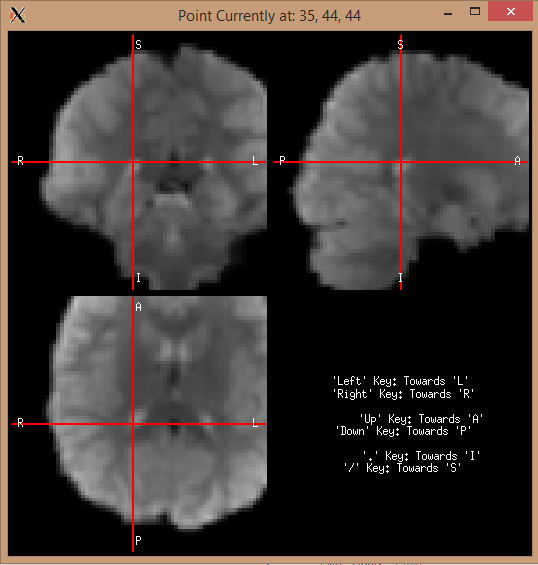
\includegraphics[width=.9\linewidth]{fig/brainconductor/50002_smooth_after.png}
\end{subfigure}%
\begin{subfigure}{.5\textwidth}
  \centering
 
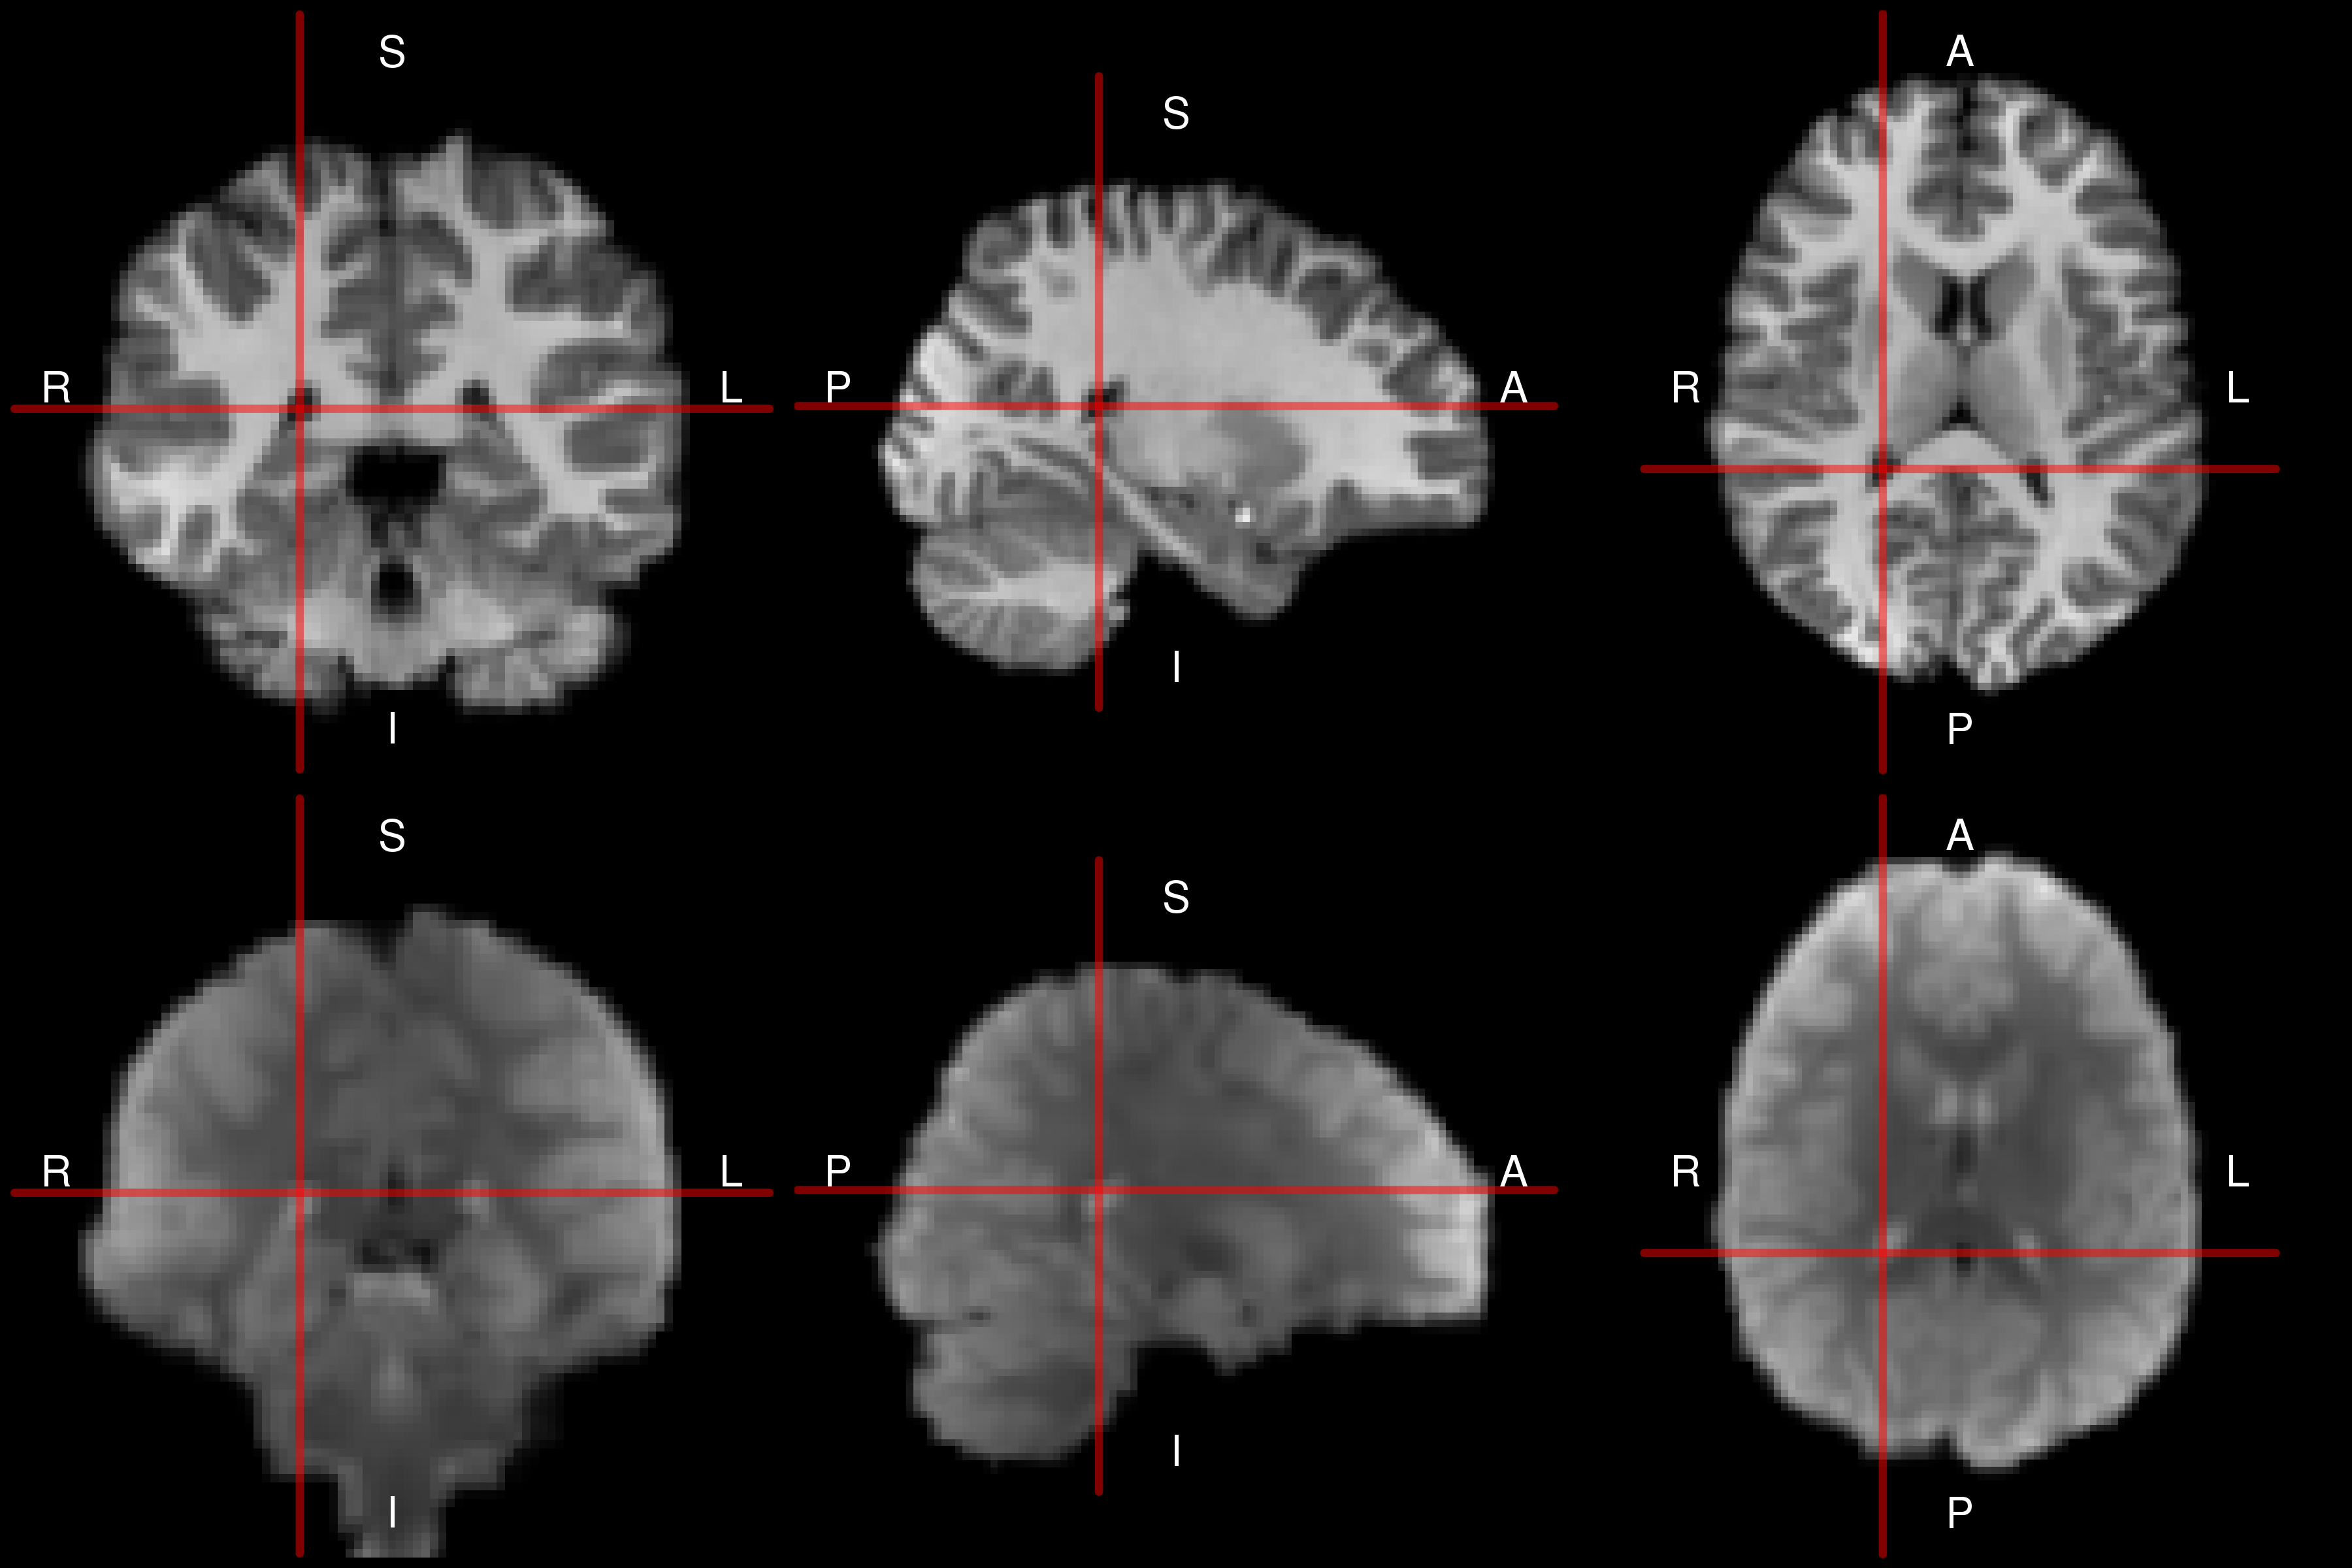
\includegraphics[width=.9\linewidth]{fig/brainconductor/50002_ventricles_20151225.png}
\end{subfigure}
\caption{(Left) BCoView, an interactive viewer in R designed to be similar to
Fslview. (Right) An alternative setting 
in BCoView to determine alignment between anatomical and functional images.
}
\label{fig:viewer}
\end{figure}

\begin{figure}
\centering
\begin{subfigure}{.5\textwidth}
  \centering
  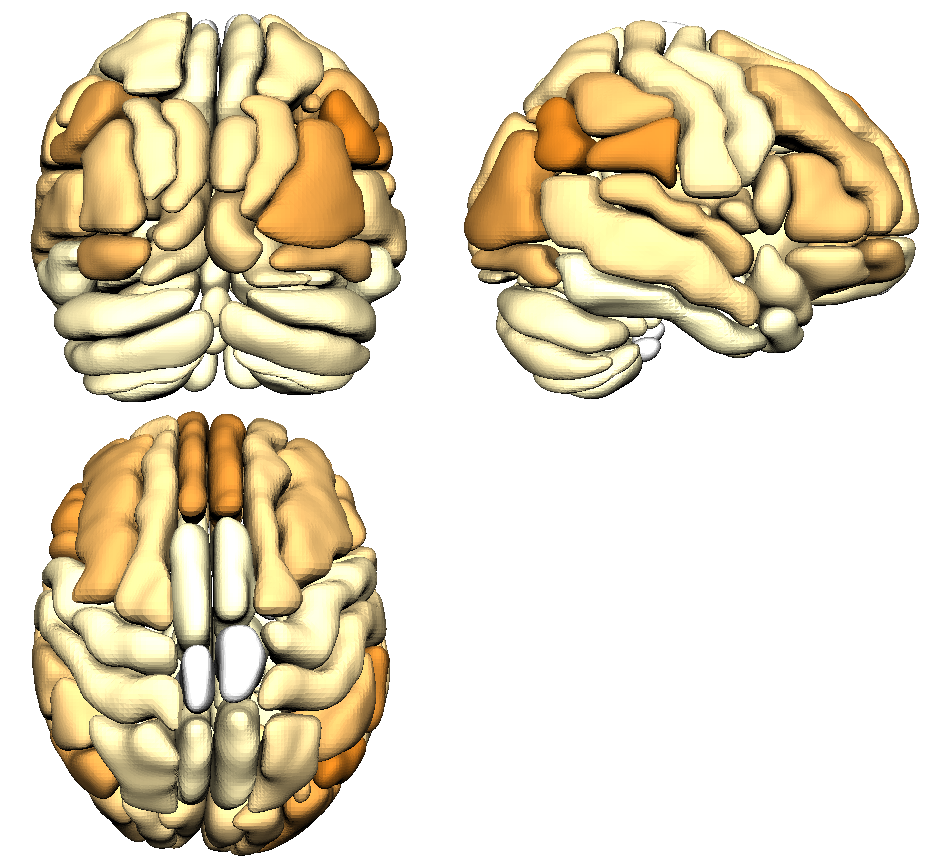
\includegraphics[width=.9\linewidth]{fig/brainconductor/AAL_all.png}
\end{subfigure}%
\begin{subfigure}{.5\textwidth}
  \centering
 
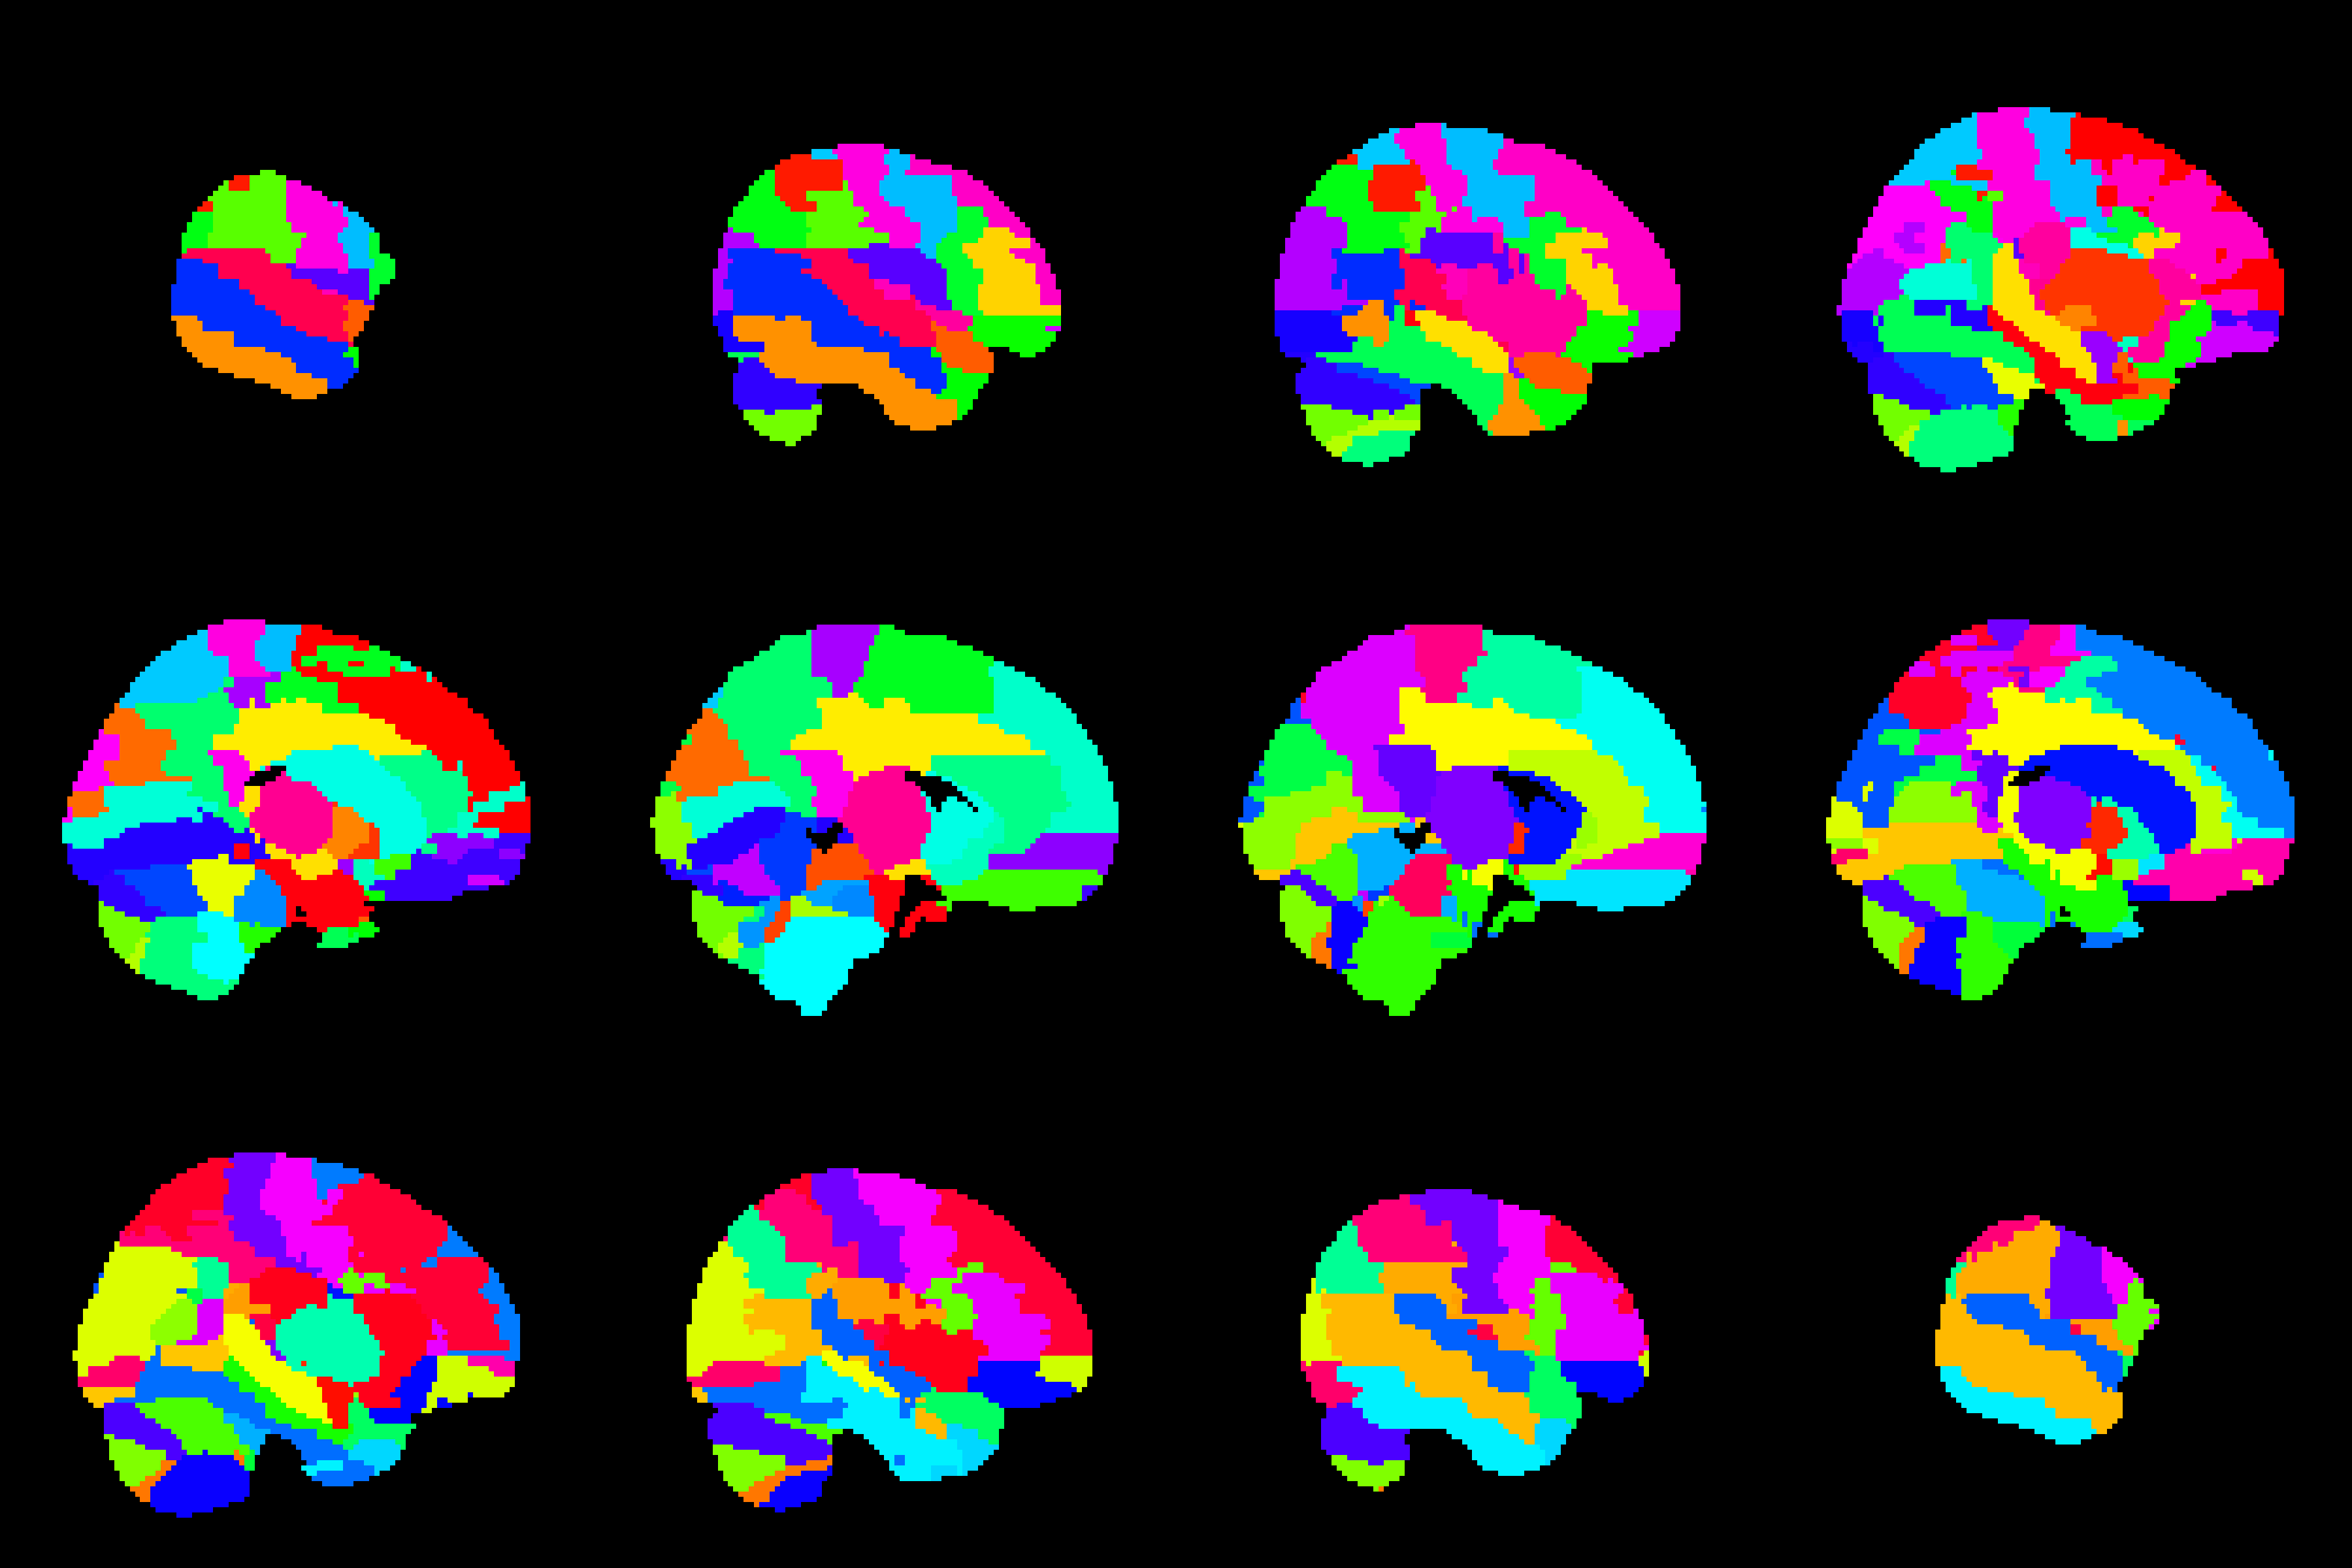
\includegraphics[width=.9\linewidth]{fig/brainconductor/partition_aal_sagittal_2016-04-11.png}
\end{subfigure}
\caption{(Left) A three-dimensional visualization of the different parcels in
AAL. (Right) A parcellation plotter in BCoViewer. Each color represents a
different parcel in AAL.}
\label{fig:aal}

\end{figure}

\begin{figure}[tb]
\centering
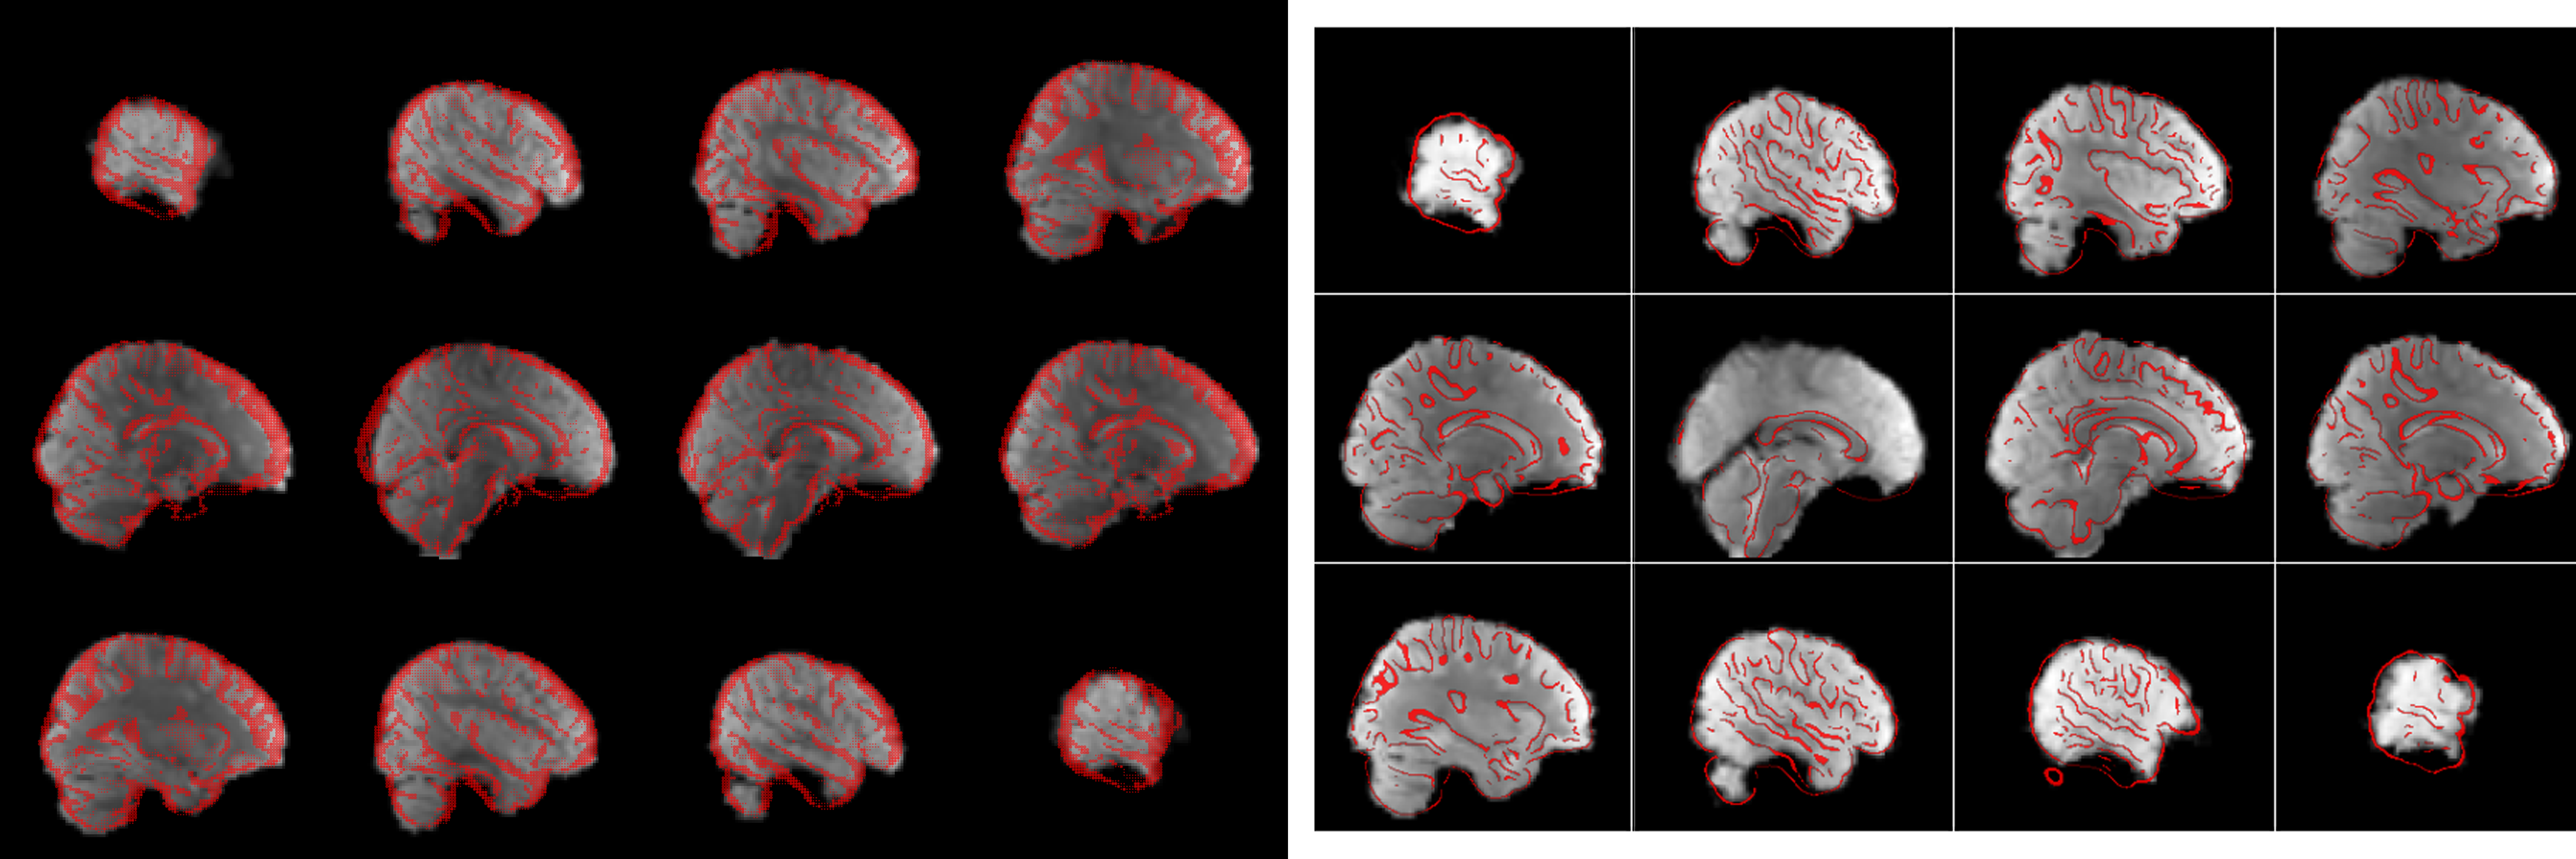
\includegraphics[width=400pt]{fig/brainconductor/comparison.png}
\caption{A comparison between our plotter in BCoViewer to visually determine how
well
a fMRI scan has been registered to the standard MNI template. Our BCoViewer
method in R
is shown on the left, while the method used in C-PAC is shown on the right. In 
both plots, the subject's functional data is shown in grayscale while the red
points/lines
trace the outline of the MNI 2mm template.}
\label{fig:overlap}
\end{figure}

In order to find the presence of abnormal functional connectivity, we 
carried out the whole-brain analysis using the Automated Anatomical
Labeling\cite{tzourio2002automated} parcellation. This divides the brain into
116 anatomical connected regions. We extracted the mean time series from each
of the 116 regions for each subject. We then performed a subject-level
connectome
analysis using neighborhood selection\cite{meinshausen2006high}. For
each subject, we chose the tuning
parameter of this method to estimate a connectome with 150 edges (roughly
sparsity
of 0.025\%). 
Based on case-control pairings matching the age, gender and IQ as closely as
possible,
we then took the graph-difference between each pair of case and control. Here,
the graph difference is represented as signed edges in one connectome but not
the other. 
We then computed the median graph\cite{han2013sparse} with 
50 edges 
to generate a population-level graph difference between the cases and controls.
The entire analysis was done using our BCoPopulation.analysis framework.

Our analysis determined that several connections within the cerebellum were
present
in controls while severed in cases. In particular, over half the case-control
pairings showed that in the control's estimated brain connectome, 
there was statistical dependency between Right lobule IV, V of the cerebellar
hemisphere (Cerebelum\_4\_5\_R) and Lobule VII of vermis (Vermis\_7) while in
the
case's estimated brain connectome, this connection was missing. A plot
of these two regions is shown in \Fref{fig:aalconnectome}. While the cerebellum
is responsible for motor learning and coordination, there is new evidence that
the cerebellum supports cognitive functions, including language and executive
functions,
as well as affective
regulation\cite{goines2011autoantibodies,braunschweig2012maternal}.
There is supporting evidence from current autism research that the cerebellum
plays
a substantial role in the development of
autism\cite{d2015cerebellar,becker2013autism,wang2014cerebellum}.

\begin{figure}[tb]
\centering
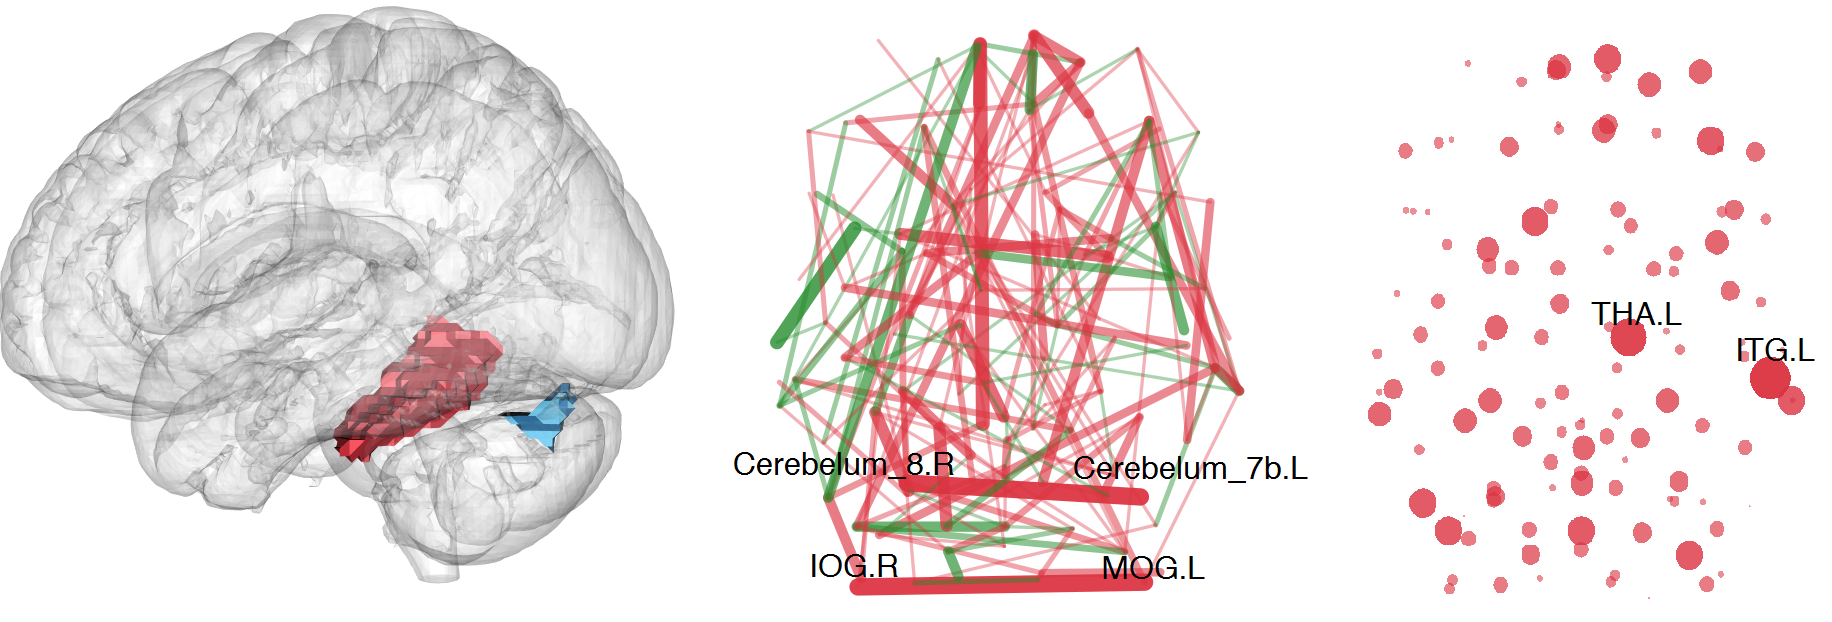
\includegraphics[width=400pt]{fig/brainconductor/aal_view_expand.png}
\caption{(Left): Perspective plot showing right lobule IV, V of cerebellar
hemisphere
(red) and Lobule VII of vermis (blue). {\color{red}include pictures of entire
graph}
(Middle): A plot of the population connectome differences plotted from
the axial view. Red edges are ones in
controls but not in autistic subjects, while green is the opposite. The
thickness of 
the line denotes how many subject-pairs displayed this connectome difference.
(Right): A plot of all 116 parcels represented by a circle where the size
of the circle denotes the degree of that parcel in the population connectome
difference.
}
\label{fig:aalconnectome}
\end{figure}

\newpage
\appendix
%
%\section{Related Tables}
%
%
%We do a comparison of the differences between Bioconductor and Brainconductor
%in \Fref{tab:bioconductor}.
%
%\begin{table}
%\begin{footnotesize}
%\begin{center}
%    \begin{tabular}{ | p{2cm} | p{6.5cm} |  p{6.5cm} |}
%    \hline
%	Main Feature & \textbf{Bioconductor} & \textbf{Brainconductor} \\ \hline
%	Data Structure Standards & ExpressionSet and SummarizedExperiment S4 classes
%based on gene data, and annotation (meta) data associated based on some common
%databases 
%	& NIdata S4 class based on imaging data and annotation (meta) data \\\hline 
%	Annotation and Resources & Provides software (BioMart) for associating
%microarray and other genomic data in real time with biological metadata from
%web databases such as GenBank, Entrez genes and PubMed (annotate package) & 
%	Provides interface DICOM, ANALYZE and NIfTI formats currently, but many other
%formats exist we
%	might not be familiar with. We currently have only specific annotation files
%(tissue priors,
%	anatomical parcellation) mostly from the standard FSL installation. \\\hline
%	Website & \url{http://bioconductor.org} & \url{http://52.69.152.114/} 
%	\\\hline
%	Reproducible Research & Advocates using Knitr & Advocates using iPython
%\\\hline
%	Testing & Automated testing of submitted packages and daily testing of
%packages & Manual testing of submitted packages \\\hline
%	Short Courses & Developed a program of short courses on software and
%statistical methods for the analysis of genomic data. & Have no courses, but
%can make if the project is successfully popularized. \\\hline
%	Maintainers & Dedicated maintainers from all over the word & Only two
%maintainers \\\hline
%    \end{tabular}
%    \caption{Contrasts between Bioconductor and Brainconductor}
%    \label{tab:bioconductor}
%\end{center}
%\end{footnotesize}
%\end{table}
%
%We list related packages that we have integrated into Brainconductor's 
%base installation. Currently, we have focused on estimate the connectome for
%fMRI data. In \Fref{tab:neuro}, we list various packages that interact with
%fMRI data. In \Fref{tab:stat}, we list various packages that estimate the
%connectome
%based on data.
%
%\begin{table}
%\begin{footnotesize}
%\begin{center}
%    \begin{tabular}{ | l | p{4cm} |  p{6cm} |}
%    \hline
%	Package Name & Full Name & Description \\ \hline
%	AnalyzeFMRI & Functions for analysis of fMRI datasets % stored in the ANALYZE
%%or NIFTI format
%	&
%	Functions for I/O, visualisation and analysis of functional Magnetic Resonance
%Imaging (fMRI) datasets stored in the ANALYZE or NIFTI format.
%	\\\hline
%	brainR & Helper functions to misc3d and rgl packages for brain imaging &
%	Includes functions for creating 3D and 4D images using WebGL, RGL, and
%JavaScript Commands \\\hline
%	fmri & Analysis of fMRI experiments &
%	Provides R-functions to perform fmri analysis \\\hline
%	fslr & Wrapper Functions for FSL  from fMRI of the Brain &
%	Wrapper functions that interface with FSL using system commands. \\\hline
%	oro.dicom & DICOM Input / Output &
%	Data input/output functions for data in the DICOM standard \\\hline
%	oro.nifti & NIfTI + ANALYZE + AFNI Input / Output &
%	Functions for the input/output and visualization of data in the ANALYZE, NIfTI
%or AFNI formats. \\\hline
%	RNiftyReg & Image Registration Using the NiftyReg Library &
%	Provides an R interface to the NiftyReg image registration tools \\\hline
%	nat & NeuroAnatomy Toolbox for Analysis &
%	Enables analysis and visualisation of 3D biological image data, especially
%traced neurons \\\hline
%	nat.templatebrains & NeuroAnatomy Toolbox Extension for Handling Template
%Brains &
%	Extends package 'nat'  by providing objects and functions for handling
%template
%brains. \\
%	\hline
%    \end{tabular}
%    \caption{fMRI Packages Incorporated into the Brainconductor Project
%%{\color{red}Why is the font different...}
%}
%    \label{tab:neuro}
%\end{center}
%\end{footnotesize}
%\end{table}
%
%\begin{table}
%\begin{footnotesize}
%\begin{center}
%    \begin{tabular}{ | l | p{4cm} |  p{6cm} |}
%    \hline
%	Package Name & Full Name & Description \\ \hline
%	bigdata & Big Data Analytics & Provides a LASSO regression using stability
%selection.
%	for large-scale data analysis \\\hline
%	camel & Calibrated Machine Learning & Provides a family of high-dimensional
%calibrated machine learning tools \\\hline
%	fastclime & A Solver for Parameterized Linear Programming to Precision Matrix
%Estimation &
%	An efficient method of recovering precision matrices by applying the
%parametric
%simplex method is provided in this package.  \\\hline
%	flare & Family of Lasso Regression &
%	Provides the implementation of a family of Lasso variants including Dantzig
%Selector, LAD Lasso, SQRT Lasso, Lq Lasso for estimating high dimensional
%sparse
%linear model. \\\hline
%	huge & High-Dimensional Undirected Graph Estimation &
%	Provides a general framework for high-dimensional undirected graph
%estimation.\\\hline
%	picasso &  Pathwise Calibrated Sparse Shooting Algorithm & Implements the
%pathwise calibrated sparse shooting algorithm regularized sparse linear
%regression, sparse logistic regression, and sparse undirected graphical model
%estimation. \\\hline
%	smart & Sparse Multivariate Analysis via Rank Transformation & Provides a
%general framework for analyzing (including estimation, feature selection and
%prediction) and visualize big data. \\\hline
%    \end{tabular}
%   \caption{Statistical Packages Incorporated into the Brainconductor Project}
%   \label{tab:stat}
%\end{center}
%\end{footnotesize}
%\end{table}

\begin{methods}
\section{Using Brainconductor.}
The current release of Brainconductor is a test version
1.0; we require R version to be above 3.1.1. Users of older R versions must
update their installation to start with Brainconductor. Download the latest
release of R, then download and install basic packages of Brainconductor by
starting R and entering the commands
\begin{lstlisting}[language = R]
> source("http://10.8.7.219/packages/BrainCo/BCoinstall.R")
> BCoInstall()
\end{lstlisting}
The BCoinstall.R script installs BrainCoSetup package. BCoInstall is a function
of BrainCoSetup package to install core packages if called by default arguments.
To install specific packages, e.g., "fmri" and "AnalyzeFMRI", call the
BCoInstall function with
\begin{lstlisting}[language = R]
> BCoInstall(c("fmri","AnalyzeFMRI"))
\end{lstlisting}
BCoInstall acquiescently installs the core packages in the MedicalImaging task
view on CRAN. Users can suppress the default installation with
\begin{lstlisting}[language = R]
> BCoInstall(installmedicalimgTV = FALSE)
\end{lstlisting}
For details of installing a CRAN task view, please see the help document of R
package "ctv".

BCoInstall also updates outdated R packages with a prompt. Users can suppress
the prompt easily using the argument ask = FALSE.

In some cases, underlying alterations in the operating system, especially in
Linux system, require recompiling all installed packages. Users can start a new
R session and enter
\begin{lstlisting}[language = R]
> source("http://Domain/BCoinstall.R")
> pkgs <- rownames(installed.packages())
> BCoInstall(pkgs, type="source")
\end{lstlisting}

Users can check packages that are either outdated or too new for their
Brainconductor version with
\begin{lstlisting}[language = R]
> library(BrainCoSetup)
> BCoValid()
\end{lstlisting}
The output provides possible solutions to identified problems, and the help page
?BCoValid shows detailed arguments and behaviours of the function.





\end{methods}

%% Put the bibliography here, most people will use BiBTeX in
%% which case the environment below should be replaced with
%% the \bibliography{} command.


\bibliography{bib}

%% Here is the endmatter stuff: Supplementary Info, etc.
%% Use \item's to separate, default label is "Acknowledgements"

\begin{addendum}
% \item Put acknowledgements here.
 \item[Competing Interests] The authors declare that they have no
competing financial interests.
 \item[Correspondence] Correspondence and requests for materials should be
addressed to Han Liu, Ph.D., Sherred Hall 224, Princeton University, Princeton,
NJ 08544 USA (email: \texttt{hanliu@princeton.edu}), and Yu Wang, Ph.D., Room
4-303, Rohm Building, E.E. Dept., Tsinghua University, Beijing, China 100084
(email: \texttt{yu-wang@tsinghua.edu.cn})
\end{addendum}

%%
%% TABLES
%%
%% If there are any tables, put them here.
%%
	
\end{document}

